\def\year{2015}
\documentclass[letterpaper]{article}
\usepackage{aaai}
\usepackage{times}
\usepackage{helvet}
\usepackage{courier}
\usepackage{graphicx}
\usepackage{url}
\setlength\titlebox{3in}
\frenchspacing
\copyrighttext{Copyright 2015, California Institute of Technology}
\setlength{\pdfpagewidth}{8.5in}
\setlength{\pdfpageheight}{11in}
\pdfinfo{
/Title (Automatic Generation of a Mars Target Encyclopedia)
/Author (Kiri L. Wagstaff, Nina Lanza, Ellen Riloff, Chris Mattmann, Paul Ramirez)}
\setcounter{secnumdepth}{2}  
 \begin{document}
% The file aaai.sty is the style file for AAAI Press 
% proceedings, working notes, and technical reports.
%
\title{Automatic Generation of a Mars Target Encyclopedia}
\author{Kiri L. Wagstaff \\
Jet Propulsion Laboratory\\
California Institute of Technology\\
4800 Oak Grove Drive, Pasadena, CA 91109\\
{\tt kiri.l.wagstaff@jpl.nasa.gov}
\And
Nina L. Lanza\\
Los Alamos National Laboratory \\
Los Alamos, NM  87545\\
{\tt nlanza@lanl.gov}
\And
Ellen Riloff\\
School of Computing\\
University of Utah\\
Salt Lake City, UT 84112\\
{\tt riloff@cs.utah.edu}
\AND
Chris A. Mattmann\\ 
\normalsize Jet Propulsion Laboratory\\
\normalsize California Institute of Technology\\
\normalsize 4800 Oak Grove Drive, Pasadena, CA 91109\\
\normalsize {\tt chris.a.mattmann@jpl.nasa.gov}
\And
Paul M. Ramirez\\
\normalsize Jet Propulsion Laboratory\\
\normalsize California Institute of Technology\\
\normalsize 4800 Oak Grove Drive, Pasadena, CA 91109\\
\normalsize {\tt paul.m.ramirez@jpl.nasa.gov}
}
\maketitle
\begin{abstract}
\begin{quote}
TBD
\end{quote}
\end{abstract}

\section{Introduction and Motivation}

The surface exploration of Mars continues to generate new data and
discoveries for an increasingly large number of targets and locations.
Mission planners and planetary science researchers must be aware of an
ever-growing number of names, locations, and facts so that new
observations can be appropriately interpreted in the context of what
is already known.  For example, one might ask: Does the observation of
high manganese content at a particular location represent a
confirmation of an existing trend or an anomalous new discovery?

The rovers that have been sent to Mars have been extraordinarily
active and productive.  The Mars Science Laboratory rover has
generated $>3500$ targets in three years, and the Mars Exploration
rover has generated even more over its 11+-year mission.  There are
hundreds of associated scientific publications reporting new
discoveries.  The downside of this productivity is that as the number
of data and publications grow, it becomes progressively more difficult
for any single person to read, understand, organize, and recollect the
amount of information available.  All researchers face the challenge
of staying up to date on new methods and advances in their field, but
Mars surface studies are particularly challenging because rather than
learning about a handful of new methods every few months or so
(through a new journal issue or a conference proceedings), the list of
new targets and discoveries grows daily.

\begin{figure}
\centerline{\fbox{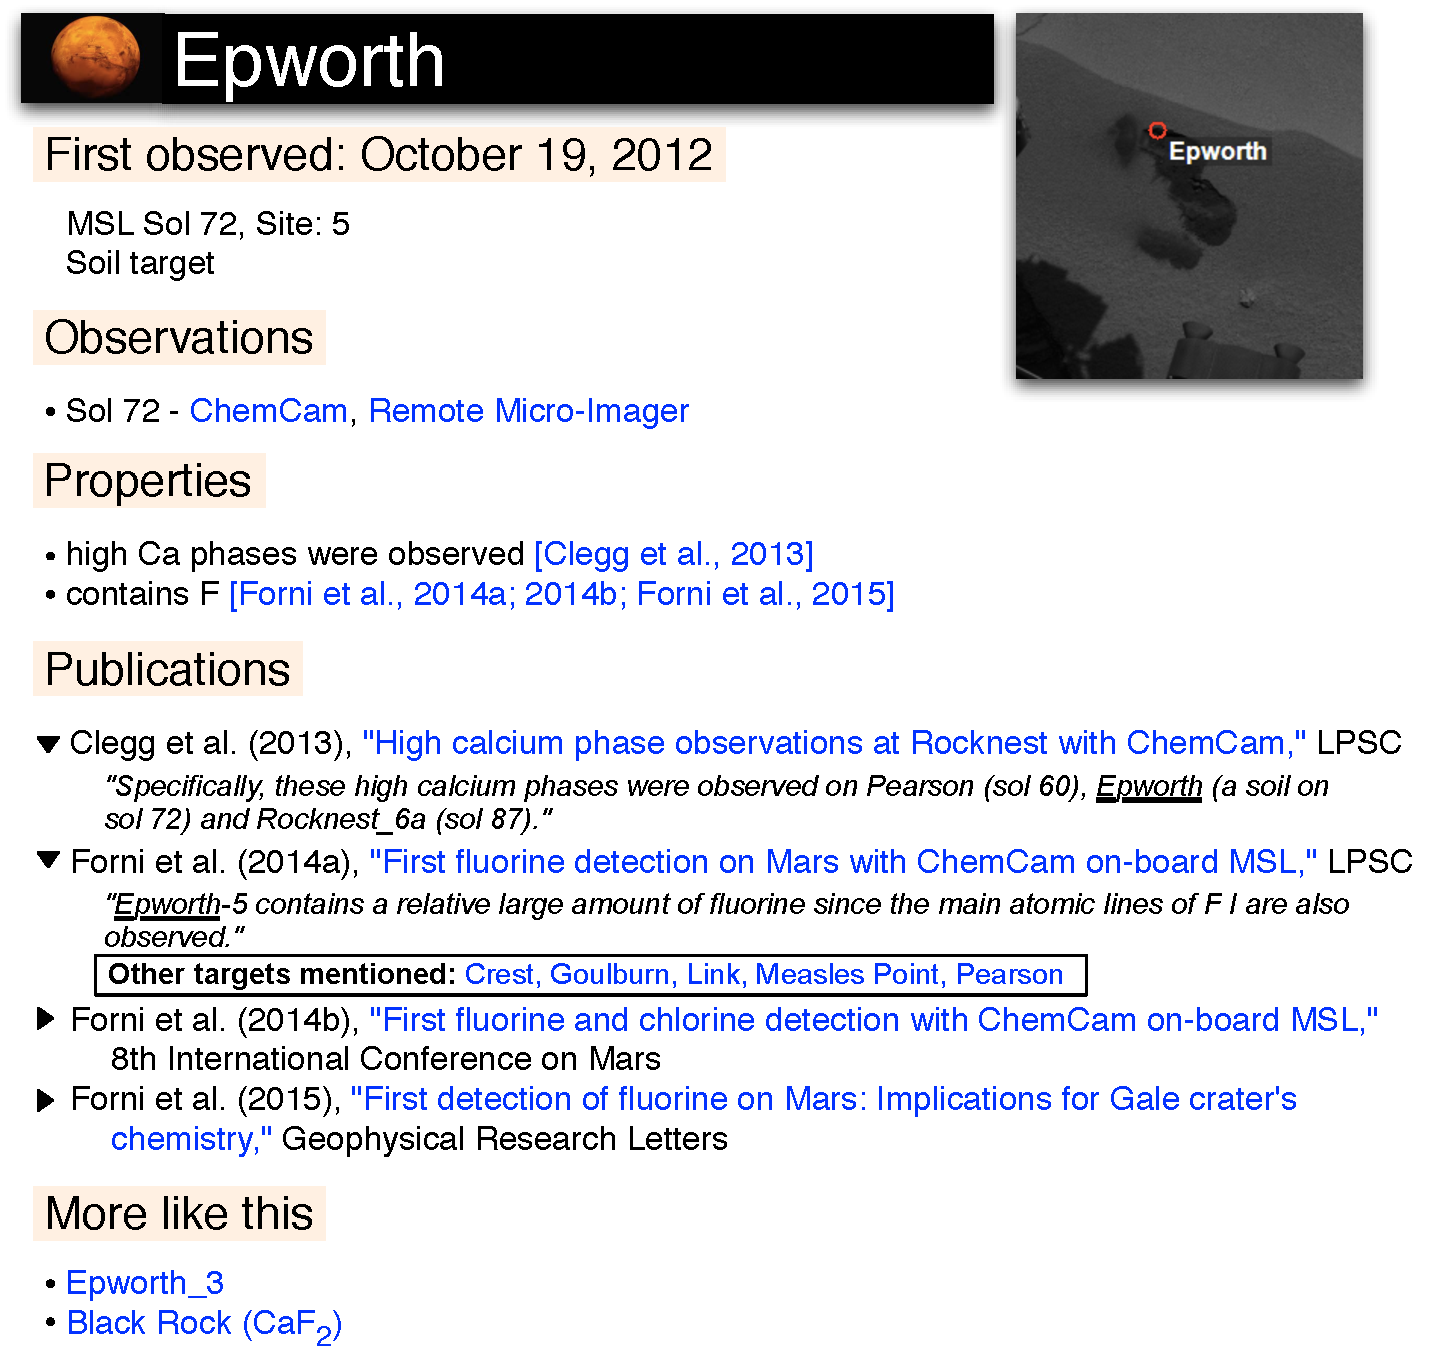
\includegraphics[width=3.25in]{fig/mte-epworth}}}
\caption{Example hand-constructed MTE entry for target
Epworth. Users can connect to the original observations, properties
that were extracted from scientific publications, and the publications
themselves.  Each publication provides excerpts with relevant context
and a list of other targets mentioned.}
\label{fig:epworth}
\end{figure}

There is a growing need for a comprehensive, up-to-date compilation of
Mars surface targets and what has been discovered about them.  The
number of targets, amount of data, and number of associated
publications are too large make this feasible as a manual task.
%
Current text search tools cannot meet the knowledge needs of planetary
scientists and mission planners.  Mars surface target names have no
naming convention, and names are often borrowed from Earth locations
(e.g.,~``Cumberland,'' ``Ithaca''), people (e.g., ``Jake'',
``Darwin''), or apparent whimsy (``Frood,'' ``Worldbeater'').  Using
Google or journal text search interfaces with these names yields many
irrelevant results.

%Volume of data: MSL - XXXX papers published in 3 years; YYYY targets
%observed by ChemCam

This situation presents an opportunity for NLP and information
extraction (IE) methods to make a major contribution that can help
advance the field of planetary science.  It also presents important
challenges that can motivate advances in IE that also benefit other
domains. 

We are working to construct a Mars Target Encyclopedia (MTE) that will
contain information about Mars surface targets.  The MTE will provide
access to the data and publications associated with each target (see
Figure~\ref{fig:epworth} for an example).  Each entry will also
include a list of properties that were automatically extracted from
the publications as a high-level summary of relevant knowledge.  The
associated excerpts will be highlighted for each publication, serving
to (1) provide support for each of the extracted properties and (2)
enable users to quickly determine which papers are of the most
interest.  Cross-document information extraction could also reveal new
connections or similarities between targets. {\bf [Cite Radev 00? Or
is this overkill?]}

\section{Constructing a Mars Target Encyclopedia}

\subsection{Data Set Description}

For our initial study, we constructed a corpus that consists of all
papers presented at the 2015 Lunar and Planetary Science
Conference (LPSC)\footnote{Downloaded
from \url{http://www.hou.usra.edu/meetings/lpsc2015/}}. 
Each of the 1,991 papers is a maximum two-page extended abstract with a
common structure: title, authors with affiliations, a two-column main
body that may contain figures and/or tables, and references.  The
language is academic and makes heavy use of complex noun phrases and
parenthentical expressions.  The passive voice is often used.
% Todo: include examples

The LPSC papers are provided in PDF format.  We used the Apache Tika
parser~\cite{mattmann:tika11} to read the PDF files and convert them to
plain text.  Four documents could not be parsed by Tika, yielding
1,987 documents.  The number of extracted words per document ranged
from 142 to 2433.

% target list
We also obtained a seed list of Mars surface target names identifed by
the ChemCam science team.  ChemCam is an instrument on the Mars
Science Laboratory (MSL) rover.  It fires a laser at rock or soil targets
and then uses a spectrometer to record the emitted energy at 6,144
wavelengths~\cite{maurice:chemcam12}.  The current list of all ChemCam
observations can be obtained
online\footnote{\url{http://pds-geosciences.wustl.edu/msl/msl-m-chemcam-libs-4_5-rdr-v1/mslccm_1xxx/document/msl_ccam_obs.csv}}.
The version we used contained 16,267 observations that spanned 656
distinct targets.

\subsection{Approach}

We used the Sundance parser~\cite{riloff:sundance04} to construct a
shallow parse of the text.  Sundance provides tokenization, sentence
segmentation, morphological analysis, part-of-speech disambiguation,
and syntactic chunking.  Because it generates basic syntactic
structures, rather than a full parse tree, Sundance can handle
sentence fragments and ungrammatical constructs.  Sundance has
previously been successfully applied to scientific publications from
the biomedical domain~\cite{ramakrishnan:bio10,pokkunuri:bio11}.  It
is also customizable for specialized domains, which allowed us to
easily tailor it for the planetary science focus of the corpus for
this project.

Our domain-specific customizations included (1) the specification of
two words that, despite ending in a period, do not indicate the end of
a sentence (``Mt.'' and ``wt.'') and (2) domain-specific vocabulary
including element names (e.g., ``chlorine'', ``Cl''), mineral names
(e.g., ``akaganeite'', ``feldspar'', ``MnO''), target names (from the
list described above), and unusual terms (e.g., ``sol'' (Martian day),
``MSL''). 

\begin{figure}
\centerline{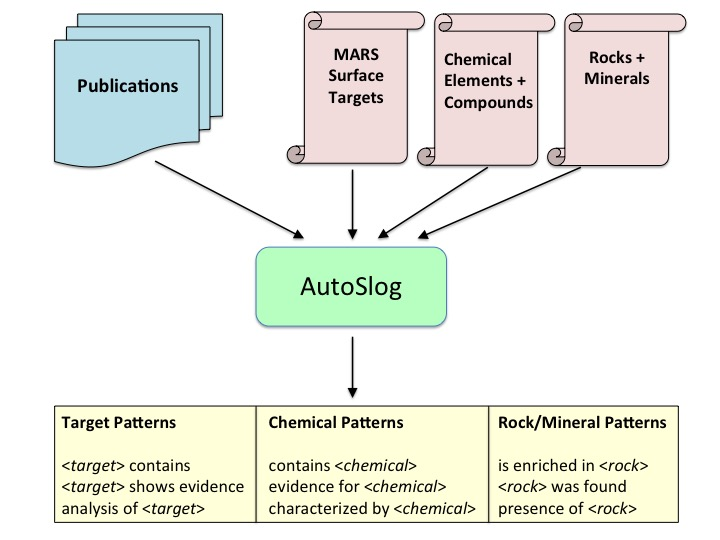
\includegraphics[width=3.5in]{fig/autoslog-process.jpg}}
\caption{The extraction pattern generation process. Autoslog learns
patterns from publications and lists of target names, chemical
elements and compounds, rocks, and minerals. {\bf [Ellen, this figure
looks a bit fuzzy - can we get a higher quality one, maybe PNG or PDF?]}}
\label{fig:ie}
\end{figure}

As shown in Figure~\ref{fig:ie}, we provide the input corpus
(publications) along with the domain-specific information to 
the AutoSlog pattern generation 
tool~\cite{riloff:autoslog93,riloff:autoslog96}.  AutoSlog  
creates extraction patterns based on the ChemCam Mars surface target
list and the way those target names appear in the parsed structure of
the LPSC documents.  These patterns are used to collect the
information that will be stored in the MTE.

\subsection{Initial Results}

In this section, we report on initial results for extracting
information for a Mars surface target named Windjana.  Windjana is a
sandstone that was named after the Windjana Gorge in Western
Australia~\cite{anderson:pads15}. 
% Cite paper 2417; this paper also has an nice image we could use

% todo: show parse output?
{\bf [Here we could show parse output (if that level of detail is
desired) and walk through one or more of 
these examples.  Which one(s) should we use?]}

{\bf [Note: I haven't yet added the element/chemical names as
extraction targets, but I could do that quickly.  Although we don't
yet have a way to automatically merge the case frames, we could show
how that would be done here.  For now I have the other info that
should be extracted in parentheses.]} 

{\em ``Windjana is remarkable in containing an abundance of potassium
feldspar (and thus K in its bulk chemistry) combined with a low
abundance of plagioclase (and low Na/K in its chemistry).''}
% cite paper 2620
Autoslog extracts:
{\tt <subj>\_CONTAINING\_ABUNDANCE} 
(of potassium feldspar)

{\em ``As in other rock samples analyzed by CheMin, Windjana contains
significant proportions of phyllosilicates and amorphous material.''}
% cite paper 2620
Autoslog extracts:
{\tt <subj>\_CONTAINS\_PROPORTIONS}
(of phyllosilicates and amorphous material)

{\em ``The high abundances of K-feldspar and iron oxides in Windjana, also
reflected in the APXS chemical analysis as high K and Fe (Table 2)
[7], are unusual.''}
% cite paper 2620
Autoslog extracts:
(K-feldspar and iron) 
{\tt OXIDES\_IN\_<subj>}

{\em ``The Windjana sandstone contains high magnetite along with 2:1
phyllosilicates [9].''}
% cite paper 2971
Autoslog extracts:
{\tt <subj>\_CONTAINS\_MAGNETITE} 
% need to know high/low!
{\bf [Note: this example is interesting because the fact that it
contains ``high'' magnetite is important (vs. ``low'' magnetite),
i.e., the adjective matters.  What should we do about that?  Is this a
future work topic?  Cardinality?  Could go with the epistemic bit
mentioned later?]}

\section{Challenges}

In addition to the typical challenges of conducting information
extraction in a new domain (e.g.,~domain-specific vocabulary), there
are several challenges of special interest involved in this project.

First, there is a need to combine case frames due to complex sentence
structure.  {\bf [hopefully we can address this, at least in example
form, above.  Or, we could keep the above examples simple and discuss
it here.]}

{\bf [Can we imagine how to handle cases like this:]} 

{\em``strong enrichment in Zn on Windjana drill fines''}

There is a need for frequent updating of the body of extracted
information, because (1) the list of Mars surface target names is
continually growing and (2) the volume of relevant publications also
grows.  

We must determine how to reconcile potential conflicting information
extracted from different authors and publications.  An interpretation
could be overturned or negated by later findings or a more careful
examination of the available data.  In all scientific endeavors,
knowledge evolves and some of it becomes outdated.  The same challenge
appears when performing information extraction for news articles {\bf
[include cites here / discuss how others address this issue]}.
%
A simple strategy would be to let the most recently reported
information, as determined by publication date, supersede older
information.  However, in some cases it is non-trivial to determine
whether two facts are consistent or contradictory.  For example,
consider two hypothetical sentences: ``Target Elinor is
feldspar-rich'' and ``Target Elinor has low Si.''  By definition, a
feldspar contains a lot of silicon, but it requires domain knowledge
to detect that these statements are in conflict.

When interpreting observations, scientific conclusions range from
solid facts to speculation about causes.  In some cases, evidence even
for basic properties (e.g., ``contains Mn'') may fall into a gray
area.  Scientific language may therefore employ epistemic modifiers
such as ``likely'' or ``probably'' or ``possibly.''  Examples from the
LPSC 2015 corpus related to the Windjana target include {\em ``the Windjana
drill tailings likely contain a spectrally opaque material (e.g.,
magnetite, ilmenite)''}~\cite{johnson:ferric15} and {\em ``the potential
presence of illite in Windjana''}~\cite{rampe:cement15}.  Distinguishing
this information from more confidently stated conclusions is vital to
preserving the nuance reported in the documents, as previously studied
in the context of medical discussion forums~\cite{sokolova:epistemic13}.
%
{\bf [Could also build on Ellen's previous work on subjective
  expressions?  (EMNLP 2003)]}

\section{Conclusions and Next Steps}

{\bf [To be fleshed out.]}

There is a need for an MTE.

We can use IE tools, plus human review/vetting, to create a reliable
resource for planetary science.

This effort benefits ongoing science investigations and the analysis of
previously collected data within full context.

We have not yet addressed the issue of coreference.

What is the role of supervision? Some human review of extracted info -
are any annotations needed? 

Describe larger planned system (store extracted information in a
Solr database, use JSON to generate MTE webpages)?

We will expand to include more text sources and ultimately targets
from other instruments/missions.

\bibliography{mte}
\bibliographystyle{aaai}

\end{document}
